% SC2203 --- Chapter 2: Regular Languages -- DFAs, NFAs, Regex (0->100 ground-up)
\chapter{Regular Languages: DFAs, NFAs and Regular Expressions}
\label{ch:regular}

\begin{quote}
\emph{``A finite automaton is the simplest computer.''} --- It reads left to right, remembers only a finite state, and decides membership. From this humble model flow NFAs, subset construction, and regexes---all equally powerful.
\end{quote}

\noindent\fbox{\parbox{\dimexpr\linewidth-2\fboxsep-2\fboxrule}{%
\textbf{From zero: we build here, no automata assumed.} We define DFA from scratch---states, transitions, extended delta---with pictures before formalism. NFAs and $\varepsilon$-moves are motivated by ``guessing''. No prior complexity is assumed; only Ch.~1 strings/languages.}}
\vspace{0.4em}

\section*{Learning Outcomes}
After this chapter you will be able to:
\begin{enumerate}[label=(L\arabic*)]
    \item define DFA formally and compute its language via $\hat\delta$;
    \item define NFA/$\varepsilon$-NFA and explain nondeterminism as existential choice;
    \item convert NFA $\to$ DFA via subset construction and argue correctness;
    \item define regular expressions and their language $L(R)$;
    \item prove Kleene's theorem: regex $\equiv$ NFA $\equiv$ DFA in expressive power.
\end{enumerate}

% ============================================================
\section{Deterministic Finite Automata}
\label{sec:dfa}
\emph{Intuition:} a turnstile that clicks through states as symbols arrive; whether you end in a green (accept) state decides membership. Only the current state matters---finite memory.

\begin{definition}[DFA]
A \emph{deterministic finite automaton} is $M=(Q,\Sigma,\delta,q_0,F)$ where $Q$ finite states, $\Sigma$ alphabet, $\delta:Q\times\Sigma\to Q$, $q_0\in Q$ start, $F\subseteq Q$ accept. Extend $\hat\delta:Q\times\Sigma^*\to Q$ by $\hat\delta(q,\varepsilon)=q$, $\hat\delta(q,wa)=\delta(\hat\delta(q,w),a)$. Language $L(M)=\{w\mid\hat\delta(q_0,w)\in F\}$.
\end{definition}

% TikZ 1: DFA for even number of 0s + code highlighting
\begin{figure}[h]
\centering
\begin{tikzpicture}[->,>=Stealth,shorten >=1pt,auto,node distance=2.2cm,semithick]
\tikzstyle{every state}=[fill=blue!12,draw=blue!60!black,thick,text=black,minimum size=1.0cm]
\node[initial,state,fill=green!18] (q0) {$q_0$};
\node[state,fill=orange!18] (q1) [right of=q0] {$q_1$};
\path (q0) edge[loop above] node {$1$} (q0)
           edge[bend left] node {$0$} (q1)
      (q1) edge[bend left] node {$0$} (q0)
           edge[loop above] node {$1$} (q1);
\node[font=\tiny,fill=yellow!12,rounded corners=2pt,inner sep=2pt] at (1.1,-1.2) {accept $=\{q_0\}$: even \# of $0$s};
\end{tikzpicture}
\caption{DFA for $L=\{w\in\{0,1\}^*\mid\#_0(w)\text{ even}\}$: state remembers parity of $0$s; $1$s loop.}
\label{fig:dfa-even0}
\end{figure}

\begin{example}[Running a DFA]
$M$ above on $w=010$: $\hat\delta(q_0,0)=q_1$, $\hat\delta(q_0,01)=q_1$, $\hat\delta(q_0,010)=q_0\in F$ so $010\in L$. On $w=0$: ends in $q_1\notin F$, reject. The table of $\delta$ is $2\times2$ entries; $\hat\delta$ is just iterated lookup.
\end{example}

\begin{example}[Code view: DFA simulator]
The transition table becomes three lines: track the current state, step it, test acceptance.
\begin{lstlisting}[language=Python]
def accepts(dfa, w):
    q = dfa.q0
    for a in w:          # deterministic: one next state
        q = dfa.delta[(q,a)]
    return q in dfa.F    # accept iff end in F
# dfa for even-zeros: Q={0,1}, delta={(0,'0'):1,(0,'1'):0,(1,'0'):0,(1,'1'):1}
\end{lstlisting}
Every DFA is a pure function $\Sigma^*\to Q$; no branching, $O(|w|)$ time.
\end{example}

% TikZ 2: Product construction intuition
\begin{figure}[h]
\centering
\begin{tikzpicture}[scale=0.75,every node/.style={font=\scriptsize}]
\draw[thick,fill=blue!10,rounded corners=4pt] (0,0) rectangle (3.6,2.0);
\node[font=\footnotesize\bfseries] at (1.8,1.7) {DFA $M_1$};
\foreach \x in {0.7,1.8,2.9} {\node[draw,circle,fill=white,minimum size=0.6cm] at (\x,1.0) {};}
\draw[->,thick,blue!60!black] (0.7,1.0)--(1.8,1.0);
\draw[->,thick,blue!60!black] (1.8,1.0)--(2.9,1.0);
\node[font=\tiny] at (1.8,0.35) {tracks $P_1$};
\draw[thick,fill=orange!14,rounded corners=4pt] (4.2,0) rectangle (7.8,2.0);
\node[font=\footnotesize\bfseries] at (6.0,1.7) {DFA $M_2$};
\foreach \x in {4.9,6.0,7.1} {\node[draw,circle,fill=white,minimum size=0.6cm] at (\x,1.0) {};}
\draw[->,thick,orange!70!black] (4.9,1.0)--(6.0,1.0);
\draw[->,thick,orange!70!black] (6.0,1.0)--(7.1,1.0);
\node[font=\tiny] at (6.0,0.35) {tracks $P_2$};
\draw[->,thick,violet!70!black] (1.8,0.02)--(1.8,-0.6)--(6.0,-0.6)--(6.0,0.02);
\node[font=\tiny,fill=green!12,rounded corners=2pt] at (3.9,-0.9) {product $Q_1\times Q_2$ tracks both};
\draw[thick,fill=green!12,rounded corners=4pt] (1.4,-2.0) rectangle (6.4,-1.1);
\node[font=\tiny] at (3.9,-1.55) {Product DFA: $(p,q)\xrightarrow{a}(\delta_1(p,a),\delta_2(q,a))$};
\end{tikzpicture}
\caption{Closure: run two DFAs in parallel via product states $(p,q)$; accept according to $F_1\times F_2$ ($\cap$), union for $\cup$, complement by flipping $F$.}
\label{fig:product-dfa}
\end{figure}

Closure under Boolean ops follows: $\overline{L(M)}$ flips $F$ to $Q\setminus F$; $L(M_1)\cap L(M_2)$ is the product DFA with $F=F_1\times F_2$; union uses $F=(F_1\times Q_2)\cup(Q_1\times F_2)$.

% ============================================================
\section{Nondeterminism and $\varepsilon$-Transitions}
\label{sec:nfa}
NFA \emph{guesses} among several next states (or $\varepsilon$-moves without consuming input); $w$ accepted if \emph{some} guess leads to accept. Surprisingly, no more powerful than DFA.

\begin{definition}[NFA and $\varepsilon$-NFA]
$N=(Q,\Sigma,\delta,q_0,F)$ with $\delta:Q\times(\Sigma\cup\{\varepsilon\})\to\mathcal{P}(Q)$. $\varepsilon$-closure $\textsc{Eclose}(S)$ = all states reachable via $\varepsilon$-only paths from $S$. Then $\hat\delta(q,\varepsilon)=\textsc{Eclose}(\{q\})$, $\hat\delta(q,wa)=\textsc{Eclose}(\bigcup_{p\in\hat\delta(q,w)}\delta(p,a))$. $w\in L(N)$ iff $\hat\delta(q_0,w)\cap F\neq\emptyset$.
\end{definition}

\begin{example}[NFA for ``ends with $01$'' is trivial nondeterministically]
States $\{q_0,q_1,q_2\}$ ($q_2$ accept); from $q_0$, on $0$ go to $\{q_0,q_1\}$ (stay or guess this is the last $01$'s $0$), on $1$ stay at $q_0$; $q_1\xrightarrow{1}q_2$. A DFA for the same language needs $3$ states anyway, but for ``$n$th symbol from end is $1$'' the NFA has $n+1$ states while DFA needs $2^n$.
\end{example}

% TikZ 3: NFA with epsilon branch
\begin{figure}[h]
\centering
\begin{tikzpicture}[->,>=Stealth,shorten >=1pt,auto,node distance=1.9cm,semithick]
\tikzstyle{every state}=[fill=violet!12,draw=violet!60!black,thick,text=black,minimum size=0.85cm]
\node[initial,state,fill=blue!12] (q0) {$q_0$};
\node[state] (q1) [right of=q0] {$q_1$};
\node[state,accepting,fill=green!16] (q2) [right of=q1] {$q_2$};
\node[state,fill=orange!14] (q3) [below of=q0,yshift=0.4cm] {$q_3$};
\path (q0) edge node {$0$} (q1)
      (q1) edge node {$1$} (q2)
      (q0) edge[loop above] node {$0,1$} (q0)
      (q0) edge[->,dashed,red!70!black] node[font=\tiny,left] {$\varepsilon$} (q3);
\node[font=\tiny,fill=yellow!12,rounded corners=2pt] at (1.9,-1.45) {$\varepsilon$-move: guess without consuming};
\end{tikzpicture}
\caption{NFA for $\Sigma^*01$ with an $\varepsilon$-shortcut illustrating nondeterministic branching; acceptance is existential over paths.}
\label{fig:nfa-epsilon}
\end{figure}

% ============================================================
\section{Subset Construction: NFA $\to$ DFA}
\label{sec:subset}
Powerset DFA $D$ simulates \emph{all} NFA possibilities simultaneously: states are subsets of $Q$.

\begin{theorem}[Subset construction]
For every NFA $N$ with $n$ states there is a DFA $D$ with $\le2^n$ states and $L(D)=L(N)$. Construction: $Q_D=\mathcal{P}(Q)$, $q_{0D}=\textsc{Eclose}(\{q_0\})$, $\delta_D(S,a)=\textsc{Eclose}(\bigcup_{p\in S}\delta(p,a))$, $F_D=\{S\mid S\cap F\neq\emptyset\}$.
\end{theorem}
\begin{proof}
Induction on $|w|$: $\hat\delta_D(q_{0D},w)=\hat\delta_N(q_0,w)$ as sets. Base $\varepsilon$ by Eclose definition. Step $wa$: $\hat\delta_D(S,wa)=\delta_D(\hat\delta_D(S,w),a)=\textsc{Eclose}(\bigcup\delta(p,a))=\hat\delta_N(q_0,wa)$. Hence $w$ reaches accept in $D$ iff some NFA path reaches $F$. \qed
\end{proof}

Blow-up is unavoidable in worst case: $L_n=\{w\mid |w|\ge n\text{ and $n$th-from-end is }1\}$ has $n+1$-state NFA but every DFA needs $\ge2^n$ states (pairwise distinguishable suffixes: Myhill--Nerode preview in Ch.~3). Subset construction is thus tight.

\begin{example}[Subset on ``ends with $01$'']
$N$ states $\{0,1,2\}$. Reachable subsets from $\{0\}$: $\{0\}\xrightarrow{0}\{0,1\}$, $\{0\}\xrightarrow{1}\{0\}$, $\{0,1\}\xrightarrow{0}\{0,1\}$, $\{0,1\}\xrightarrow{1}\{0,2\}$ accept, $\{0,2\}\xrightarrow{0}\{0,1\}$, $\{0,2\}\xrightarrow{1}\{0\}$---$4$ reachable of $8$ possible.
\end{example}

% ============================================================
\section{Regular Expressions}
\label{sec:regex}
Regexes are syntax for regular languages.

\begin{definition}[Regex and $L(R)$]
Basis: $\emptyset$, $\varepsilon$, $a$ for $a\in\Sigma$ with $L(\emptyset)=\emptyset$, $L(\varepsilon)=\{\varepsilon\}$, $L(a)=\{a\}$. Inductive: if $R_1,R_2$ regex then $(R_1+R_2)$, $(R_1R_2)$, $(R^*)$ with $L(R_1+R_2)=L(R_1)\cup L(R_2)$, $L(R_1R_2)=L(R_1)L(R_2)$, $L(R^*)=L(R)^*$. We write $+$ for union, omit $\cdot$ for concat, $R^+=RR^*$, $R^?=R+\varepsilon$.
\end{definition}

\begin{example}[Regex shorthands]
Over $\{0,1\}$: $(0+1)^*$ = $\Sigma^*$; $(0+1)^*01$ = ends with $01$; $(0+1)^*01(0+1)^*$ = contains $01$; $0^*1^*$ = some $0$s then some $1$s ($\neq(0+1)^*$). Note $a^*$ vs.\ $a^+$ vs.\ $a^?$.
\end{example}

% Encoding regex to NFA is Thompson construction; NFA to regex is state elimination.

% ============================================================
\section{Kleene's Theorem: Regex $\equiv$ NFA $\equiv$ DFA}
\label{sec:kleene-thm}
\begin{theorem}[Kleene, 1956]
$L$ is regular (DFA-recognisable) iff it is denoted by some regex, iff it is recognised by some NFA/$\varepsilon$-NFA. Conversions are effective.
\end{theorem}
\begin{proof}[Sketch]
DFA$\Rightarrow$NFA trivial (deterministic is special case). Regex$\Rightarrow\varepsilon$-NFA by Thompson: build inductively for $\emptyset,\varepsilon,a$ (2-state fragments) then compose with $\varepsilon$-branches for $+$, chain for $\cdot$, loop for $*$. NFA$\Rightarrow$DFA is subset construction. DFA$\Rightarrow$regex by state elimination: generalise transitions to regex labels and rip out states one by one, replacing $p\xrightarrow{R_1}q\xrightarrow{R_2}r$ plus loop $R_3$ at $q$ with $p\xrightarrow{R_1R_3^*R_2}r$ and $p\xrightarrow{R_1R_3^*R_2+R_4}r$ if direct $R_4$ exists. \qed
\end{proof}

\begin{example}[DFA$\to$regex on even $0$s]
Eliminate $q_1$ from Fig.~\ref{fig:dfa-even0}: loop on $q_0$ labelled $1+01^*0$? Instead systematic: start with $2$-state GNFA, eliminate $q_1$: self-loop $1$ at $q_1$, $q_0\to q_1$ on $0$, $q_1\to q_0$ on $0$, so after elimination $q_0$ gets $1+0(1)^*0$? Actually $1^*0(1^*0)^*$? Simpler: regex $1^*(01^*01^*)^*$. Tools automate; key is existence.
\end{example}

\begin{remark}[Thompson in code]
Thompson's inductive step is literally an AST walk:
\begin{lstlisting}[language=Python]
def thompson(node):
    if node.kind=='lit': return fragment(node.char)      # 2 states
    if node.kind=='concat': return concat(thompson(node.left), thompson(node.right))
    if node.kind=='union':  return union(thompson(node.left), thompson(node.right))  # epsilon fork
    if node.kind=='star':   return star(thompson(node.child))  # epsilon loop
\end{lstlisting}
Each combinator adds at most $2$ new states and $\varepsilon$-edges, so size is linear in $|R|$. Epsilon-closure then costs $O(|Q|+|\delta|)$ per step.
\end{remark}

% ============================================================
\section{Chapter Notes}
Rabin and Scott introduced NFAs and subset construction (1959); Kleene linked regexes to automata (1956). Brzozowski derivatives give an alternative regex$\to$DFA.
Closure properties make regular languages a Boolean algebra; the product and subset constructions are reused for intersection, complement, and decidability in Ch.~3.
For implementation, prefer Thompson + subset lazily (\texttt{on-the-fly}) to avoid the $2^n$ blow-up unless minimised.
Aho--Sethi--Ullman (Compilers) gives the industrial Thompson implementation used in \texttt{grep}.

% ============================================================
\section{Exercises}
\label{sec:ch02-exercises}
\begin{enumerate}[label=E2.\arabic*, leftmargin=*, itemsep=0.8em]
\item \textbf{DFA table.} Build DFA for $L=\{w\mid w$ contains $010$ as substring$\}$ with $4$ states. Give $\delta$ table, identify trap, and trace $w=00101$.
\item \textbf{NFA to DFA.} Convert NFA for ``ends with $01$'' via subset construction; list all $4$ reachable subsets and draw resulting DFA. Is it already minimal?
\item \textbf{Regex to $\varepsilon$-NFA.} Thompson-construct $\varepsilon$-NFA for $(a+b)^*abb$; count states before and after $\varepsilon$-removal, then simulate on $ababb$.
\item \textbf{Distinguishing power.} Prove $L_n$ ($n$th-from-end is $1$) needs $n+1$-state NFA but $\ge2^n$ DFA states: show $2^n$ suffixes $x_i$ pairwise distinguishable by some $z$.
\item \textbf{State elimination.} Eliminate states on DFA with $Q=\{q_0,q_1,q_2\}$, $q_2$ accept, transitions $q_0\xrightarrow{a}q_1$, $q_1\xrightarrow{b}q_2$, $q_1\xrightarrow{a}q_1$, $q_0\xrightarrow{b}q_0$, to obtain regex for $b^*ab^*?a(a+b)^*$ variant; verify on $aab$.
\end{enumerate}
% End of Chapter 2
